\chapter{Introduction}
\label{sec:introduction}

Since the invention of modern computers Monte Carlo methods have become a frequently applied tool for challenging numerical problems in a wide variety of fields ranging from chemical physics to financial econometrics. With the proceeding evolution of computers, the complexity of the treated problems is growing even faster and Monte Carlo methods are now expected to deal with high dimensionalities and more and more complex structures. Hence, the computational complexity of these methods is  a crucial question nowadays.

Monte Carlo methods constitute a broad class of computational algorithms that generally rely on the principle of repeated random sampling to solve a numerical problem. The subclass of Markov chain Monte Carlo (MCMC) algorithms~\autocite{Robert2005}  performs the sampling from complex probability distributions in high dimensions by generating a Markov chain, which has the desired probability distribution as its equilibrium distribution. In many situations this is a suitable and efficient strategy to solve emergent problems in applications~\autocite{Liu2004, Robert2005}. It is therefore of interest to analyze the structure inherent to these algorithms in order to understand their computational complexity. This is most naturally undertaken by examining the behavior of the method on a family of probability distributions indexed by a parameter and then studying the cost of the algorithm as a function of that parameter. As a fruitful way to do this, the theory of  diffusion limits for MCMC methods in high dimensions is an established approach and provides a useful theoretical tool for studying the computational complexity. In particular, we will study these algorithms applied to  distributions derived from finite-dimensional approximations of a measure on an infinite-dimensional space. This setting arises in widely used applications such as Bayesian nonparametric statistics or conditioned diffusion~\autocite{Beskos2008, Beskos2009, Dashti2012, Dashti2013, Delyon2006, Hairer2011, Stuart2010}.
\newline

Our interest is focused on Metropolis-Hastings MCMC methods. We study the Random Walk Metropolis algorithm (RWM) and the Metropolis-adjusted Langevin algorithm (MALA)~\autocite{Liu2004, Robert2005}. The Metropolis-Hastings~(MH) methodology is simple but effective. To generate samples from a $N$-dimensional target density $ \pi^{N} $, a Markov chain  is constructed according to a random walk. For this,  a two-step algorithm is used. First,  a candidate according to an arbitrary transition rule is generated. In a second step, this candidate or proposal is rejected with a certain probability such that the resulting Markov chain will be $\pi^N$-invariant. While the second acceptance-rejection step, often called 'metropolizing' is fixed, the choice of a suitable proposal is free. Two widely used proposals are the random walk proposal (obtained from
the discrete approximation of Brownian motion)
\begin{equation}
\label{RWM-proposals-simple} 
  y = x + \sqrt{2\delta}\,Z^{N}, \qquad Z^{N} \thicksim \mathcal{N}\left( 0,I_N \right),
\end{equation}
and the Langevin proposal (obtained from the time discretization of the
Langevin diffusion)
\begin{equation}
\label{MALA-proposals-simple}
  y = x +  \delta \nabla \log \pi^{N} (x) + \sqrt{2\delta} Z^N, \qquad Z^{N} \thicksim \mathcal{N}\left( 0,I_N \right).
\end{equation}
Here $ 2 \delta $ is the proposal variance, a parameter quantifying the size of the discrete time increment. We will consider “local proposals” for which $ \delta $ is
small and note that $ \delta $ will depend on the dimension $N$, i.e., $\delta  = \delta(N) $. 

Equations~(\ref{RWM-proposals-simple}) and~(\ref{MALA-proposals-simple}) can be also expressed in terms of transition kernels~$q(x,y)$. Now, through metropolizing some candidates are rejected according to the following rule: from the current state $ x $, we propose $ y $ drawn from the kernel $ q(x, y) $; this is then accepted with probability
\begin{equation}
\label{acceptance probability simple}
 \alpha^{N}(x,y)  := 1 \wedge \dfrac{\pi^{N}(y) q(y,x) }{\pi^{N}(x) q(x,y)}
\end{equation}
and otherwise rejected. Here $ a \wedge b := \min (a,b)$. The Markov chain corresponding to the proposal given in Equation~(\ref{RWM-proposals-simple}) is the RWM algorithm~\autocite{Metropolis1953}, and the Markov transition rule constructed from the proposal defined in Equation~(\ref{MALA-proposals-simple}) is known as the MALA algorithm~\autocite{Robert2005}.

\begin{figure}%[htb]
 \begin{center} 
  \includegraphics[width=0.6\textwidth]{figure_2}
  \vspace*{1mm}
  \subcaption{Too small proposal variance with strong dependences.}
  \label{fig:3DscatterplotRWM-small}
  \vspace*{3mm}
  \includegraphics[width=0.6\textwidth]{figure_3}
  \vspace*{1mm}
  \subcaption{Too large proposal variance causes too much rejected movements.}
  \label{fig:3DscatterplotRWM-large}
  \vspace*{3mm}
  \includegraphics[width=0.6\textwidth]{figure_1}
  \vspace*{1mm}
  \subcaption{'Optimal scaled' RWM algorithm with a good mixing between both modes.}
  \label{fig:3DscatterplotRWM-optimal}
 \end{center}
  \caption{5000 samples produced by a RWM algorithm of a multimodal non-product target density. 1000 consecutive samples are always labeled in the same color.}
  \label{fig:3DscatterplotRWM}
\end{figure}

Let us now consider an heuristic argument for an optimal scaling of these Metropolis-Hastings algorithms via the proposal variance~$\delta(N)$. In Figure~\ref{fig:3DscatterplotRWM}, the optimal scaling characteristic of Metropolis-Hastings methods is illustrated by a Random Walk Metropolis-Hastings algorithm. The first 5000 samples produced by a RWM algorithm applied to a multimodal non-product target measure in dimension $N=10$ are depicted. Moreover, every 1000 consecutive samples are labeled in the same color to better illustrate the movement of the generated chain. These sample chains generated by the RWM (or MALA) algorithm should ideally be not correlated, as strong dependences in the samples leads to poor MCMC estimates. Hence good mixture of the colors in Figure~\ref{fig:3DscatterplotRWM} visualizes fewer dependences between the samples and vice versa. 

\begin{figure}[htb]
\begin{center}
  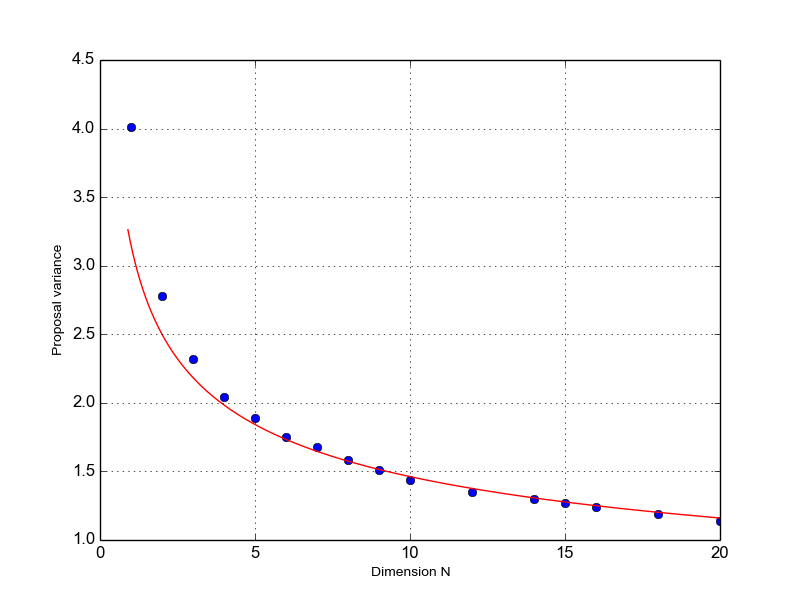
\includegraphics[width=0.7\textwidth]{proposalvariancesForDimensions}
\end{center}
  \caption{Proposal variances~$\delta$ for a MALA algorithm applied to a standard Gaussian distribution such that the mean average acceptance rate~$\alpha$ of the simulation is approximately 0.50 (blue). As comparison, the function $F(N) = 3.15 \; N^{-1/3}$ is given (red).}
  \label{fig:proposalVarianceForDimensions}
\end{figure}

A simple numerical simulation as in Figure~\ref{fig:3DscatterplotRWM} illustrates that too small or large proposal variances result in a poor performance of the algorithm. For extremely small proposal variances (see Figure~\ref{fig:3DscatterplotRWM-small}), the algorithm will propose only small jumps and almost every step will be accepted. Thus, the average acceptance rate is almost one. However, the size of the proposed jumps is too small to explore the target distribution rapidely. The convergence of the algorithm to its stationary distribution will take too long. In the case of too large proposal variances, the algorithm will propose large jumps, i.e., to far distant regions. It will therefore reject most of its proposed moves and the Markov chain stays in single states for a long period of time. It seems reasonable that there exist 'good' intermediate values for the proposal variance (see Figure~\ref{fig:3DscatterplotRWM-optimal}). This behavior is observable for every dimension $N$.

However, such 'optimal' intermediate proposal variances $ \delta(N) $ seem to decrease with increasing dimension $N$. In Figure~\ref{fig:proposalVarianceForDimensions}, we have applied the MALA algorithm to a standard Gaussian distribution for different dimensions~$N$ and plotted the proposal variance~$\delta$ such that the mean acceptance probability for 10,000 iterations is approximately 0.50. For better comparison, we plotted the function $F(N) = 3.15 \cdot N^{-1/3}$ in the same diagram. The scaling~$N^{- 1/3}$ was shown to be optimal for product measures such as Gaussian measures in previous works~\autocite{Roberts1997, Roberts1998}. A similar behavior can be observed for non-product measures.

\subsection*{Statement of the problem}

The structure of the Metropolis-Hastings methods introduced above is rather simple. At each step a move is proposed according to Equation~(\ref{RWM-proposals-simple}) or~(\ref{MALA-proposals-simple}) and this candidate is accepted with a certain probability given in Equation~(\ref{acceptance probability simple}). These quantities depend on the target distribution $ \pi^{N} $ and the proposal kernel $ q(x,y) $, which is characterized by the proposal variance $ \delta(N) $ in the case of Gaussian jumps. Therefore all occurring quantities can be indexed by a parameter; in this case the dimension $N$. It is our aim to study the cost as a function of dimension for the RWM and MALA algorithm applied to different families of probability distributions. Early results~\autocite{Roberts1997, Roberts1998} concerned product measures for which an optimal scaling via diffusion limits for RWM and MALA was obtained. It was shown that the computational complexity of the RWM method  is $\mathcal{O}(N)$ for an average acceptance rate of 0.234~\autocite{Roberts1997} when started in stationarity and applied to simple product distributions. Similarly, the cost of the MALA method, started in stationarity and applied to simple product distributions, was characterized as $\mathcal{O}(N^{1/3})$ for an average acceptance rate of 0.573~\autocite{Roberts1998}. These results were  extended to a slightly wider class of target measures but they all had in common that the diffusion limits obtained remain essentially one dimensional~\autocite{Bedard2007, breyer2004, Christensen2003}. In 2010,  Mattingly, Pillai and Stuart~\autocite{Mattingly2010} analzyed the RWM algorithm applied to finite-dimensional approximations of measures obtained from Gaussian measures in infinite dimensional Hilbert spaces by a change of measures.  The analysis for the MALA algorithm in the same setup was treated by Pillai, Stuart and Thi\'{e}ry~\autocite{Pillai2012} in 2012. Both diffusion limits are given through an infinite dimensional stochastic differential equation. Nevertheless, the results for the computional complexity as well as the optimal acceptance rate obtained in the product case extend to this Hilbert space setup. This specific setting occurs in widely used applications such as Bayesian nonparametric statistics with Gaussian priors and conditioned diffusion with additive noise~\autocite{Beskos2009, Stuart2010}. 

In this work we want to adapt the RWM results of Mattingly, Pillai and Stuart~\autocite{Mattingly2010} to the proof strategy used in Pillai, Stuart and Thi\'{e}ry~\autocite{Pillai2012} for the MALA method. In both works, they proved an optimal scaling result of the respective MCMC method by a similar diffusion limit ansatz for the same infinite dimensional Hilbert space setup. But in the estimation of the error terms they used different approaches such that they are not directly transferable. More precisely, we will combine and summarize the methods from~\autocite{Mattingly2010} and~\autocite{Pillai2012} to prove a diffusion limit result for RWM and MALA in the above Hilbert space setting simultaneously, where the speed of the interpolant of the generated Markov chains and the proposal variance of the RWM or MALA candidates scales in the correct sense. This diffusion limit result enables us to quantify the computational cost or efficiency uniquely. Theoretically, this statement holds only asymptotically. As we will see in Chapter~\ref{Numerical Results}, it seems reasonable for these asymptotic results to hold for finite dimensions, too. This point of view is supported by several numerical studies~\autocite{Beskos2008, Gelman1996, Roberts2001}.



\subsection*{Own contributions}

The contribution of this work is three-folded and emphasized in the following.
\begin{itemize}
 \item The main contribution of this Master thesis is the adaption of the proof strategy introduced by Pillai, Stuart and Thi\'{e}ry~\autocite{Pillai2012} for the MALA algorithm to the RWM algorithm analyzed from Mattingly, Pillai and Stuart~\autocite{Mattingly2010}. On the one hand, both algorithms are applied to the same class of target measures supported on an infinite dimensional Hilbert space and both works derive a diffusion limit result using the same general arguments. On the other hand, they differ in several key estimates. As the structure of both algorithms is similar in the analyzed setting, we want to emphasize this common structure by proving a diffusion limit result simultaneously for both algorithms. Nevertheless, some minor technical estimates have to be treaten separately. Since the argumentation of~\autocite{Pillai2012} is cleaner, we adapt the proof for the RWM algorithm given in~\autocite{Mattingly2010}. This is mainly expressed in the statements of Chapter~\ref{sec:DLR-Estimates}, especially in Lemma~\ref{DLR: Lemma Gaussian approximation}, Lemma~\ref{DLR: Lemma Dirft approximation} and Lemma~\ref{DLR: Lemma Noise approximation}. However, we tried to improve the comprehension by filling minor gaps in the argumentation and reorganizing some statements, particularly in Section~\ref{sec:DLR-Preliminaries}, Section~\ref{sec:sub:DLR-Proof strategy} and Section~\ref{sec:sub:DLR-General diffusion approximation}. Moreover, we resolved an inconsistency in~\autocite{Pillai2012}, see Remark~\ref{DLR-Remark Change of basis}. Therefore, we are able to state the main Theorem~\ref{DLR-THM main theorem} by using only one covariance operator and not two.
 \item Since MCMC methods are a point of intersection between statistics and probability theory, it is in some aspects difficult to receive a comprehensive overview. Thus, we compiled an outline in Chapter~\ref{ch:Computational Complexity} summarizing the ideas of computional complexity and efficiency of MCMC methods and giving an answer to the question why diffusion limits are a suitable approach to measure the computational complexity of these methods.
 \item Finally, we have done several numerical studies in Chapter~\ref{Numerical Results}. A RWM and a MALA algorithm have been implemented in the coding language \textit{python}. For different target probability distributions several statistical tests have been performed. They indicate that the theoretical and asymptotic results in the precedent chapters hold in practice and in particular, in finite dimensional settings, see Section~\ref{sec:sub:Numericals Non-product targets} and Section~\ref{sub:sec:Numericals Low dimensions}. Furthermore, the practical enhancement of the MALA algorithm in comparison to the RWM algorithm is illustrated, see Section~\ref{sec:sub:Numericals: Comparison MALA - RWM}.
\end{itemize}


\subsection*{Outline}

In Chapter~\ref{sec:Metropolis-HastingsMethod} we will introduce the Metropolis-Hastings methodology rigorously. Especially, convergence and ergodicity properties of the general Metropolis-Hastings algorithm are presented. Additionally, the two frequently used variants of the MH algorithm, the Random Walk Metropolis algorithm and the Metropolis adjusted Langevin algorithm are described.

Chapter~\ref{ch:Computational Complexity} comprises a brief introduction in the theory of computational complexity and describes different ways to measure complexity in the case of MCMC methods. This will  allow us to scale the algorithm in such a way that the complexity is minimal.We will call such a scale optimal. To complete the picture of complexity, we give an overview on existing optimal scaling results for the RWM and MALA algorithm. 

In Chapter~\ref{Application} two main applications of the RWM and MALA algorithm are given: conditioned diffusions and Bayesian nonparametric statistics. 

Chapter~\ref{Diffusion Limit Results} contains statement and proof of the main theorem of this work. According to Mattingly, Pillai and Stuart~\autocite{Mattingly2010} and Pillai, Stuart and Thi\'{e}ry~\autocite{Pillai2012}, we state a diffusion limit result indicating that the optimal scaling of RWM and MALA  for target distributions found from finite-dimensional approximations of a measure on an infinite-dimensional Hilbert space is $\mathcal{O}(N)$ and $\mathcal{O}(N^{1/3})$, respectively. 

Finally, Chapter~\ref{Numerical Results} gives a numerical study suggesting that the asymptotic results in the previous chapters hold in finite dimensions.


%\subsection*{Acknowledgements}

%A list of persons, who deserve my acknowledgements: advisor, parents, friends.



